%---------- Inleiding ---------------------------------------------------------

\section{Introductie}%
\label{sec:introductie}

In het begin van 2023, op 6 januari, werd de NIS-richtlijn, wat staat voor "Network and Information Security", opgevolgd door zijn nieuwe versie, NIS2.
Deze update bracht verschillende nieuwe voorschriften met zich mee op het gebied van cyberbeveiliging, en het aantal sectoren dat aan deze richtlijnen moet voldoen, werd aanzienlijk uitgebreid.

De lidstaten van de Europese Unie hebben tot oktober 2024~\autocite{NIS2Directive2022} de tijd om deze nieuwe richtlijnen in hun nationale wetgeving te implementeren.
Dit geeft bedrijven een beperkte periode om hun processen aan te passen aan deze nieuwe wetgeving, een uitdaging die vooral voor kleine of middelgrote ondernemingen (KMO's) problematisch kan zijn, gezien hun vaak beperkte middelen.

Een van de essenti\"ele vereisten van deze richtlijnen is dat bedrijven verplicht zijn om een ``inventory of assets'' op te stellen voor alle systemen en operaties die ze gebruiken.
Deze bachelorproef richt zich specifiek op het bieden van een oplossing voor KMO's, binnen sectoren die nu wel moeten voldoen aan deze richtlijnen, voor het inventariseren van Linux-systemen hun configuratie, waarbij de focus ligt op het vergemakkelijken van het naleven van deze nieuwe regelgeving.

Om dit te bereiken, zal een script of tool worden ontwikkeld die automatisch op elke Linux-server kan worden uitgevoerd, en gekeken worden naar reeds bestaande oplossingen die we kunnen gebruiken.
Deze tool biedt vervolgens een gedetailleerde inventaris van het systeem en de configuratie van verschillende applicaties.
Het uiteindelijke doel is om deze tool uit te voeren op vijf verschillende servers met specifieke use cases.
Op basis hiervan zal worden geconcludeerd of het implementeren van deze tool nuttig is voor KMO's.

%---------- Stand van zaken ---------------------------------------------------

\section{Literatuurstudie}%
\label{sec:litaratuurstudie}

Volgens een studie uit 2022~\autocite{Kotenko2022} is het opstellen van een configuratie inventaris essentieel voor het beoordelen van cybersecurityrisico's.
Aan de hand van een inventaris kan men potenti\"ele kwetsbaarheden gaan identificeren en de passende maatregelen gaan treffen.
Ook wordt er benadrukt dat de invenaris kan gebruikt worden om mogelijke cyberaanvalspaden te identificeren en het voorkomen van verliezen door cyberaanvallen.
Het regelmatig herevalu\"eren van de invenaris wordt benadrukt als een proactieve benadering om potenti\"ele incidenten te voorkomen.
Dit benadrukt het belang van een nauwkeurige inventarisatie voor het implementeren van geautomatiseerde detectie- en bewakingsmaatregelen.

In een boek geschreven door Antal~\autocite{Antal2010} worden verschillende systeemeigenschappen genoemd die essentieel zijn voor een inventaris.
Hoewel het boek niet specifiek gericht is op Linux-systemen, biedt het een algemeen overzicht van cruciale aspecten van een inventaris.
Hierbij wordt de configuratie van het besturingssysteem benadrukt, inclusief details zoals de kernel- en besturingssysteemversie.
Verder wordt het belang van het aantal geïnstalleerde applicaties en hun configuratie benoemd als significant in het inventarisatieproces.
Daarnaast wordt de netwerkconfiguratie, waaronder IP-adressen en firewallconfiguratie, als essentieel beschouwd.

%---------- Methodologie ------------------------------------------------------
\section{Methodologie}%
\label{sec:methodologie}

In deze studie wordt onderzoek gedaan naar de bijdrage van een configuratie-inventaris van Linux-systemen aan het initi\"ele proces van incident response bij een cyberaanval.
Het onderzoek zal bestaan uit zes fasen, zoals weergegeven in figuur~\ref{fig:flowchart}.

\begin{figure}[h!]
    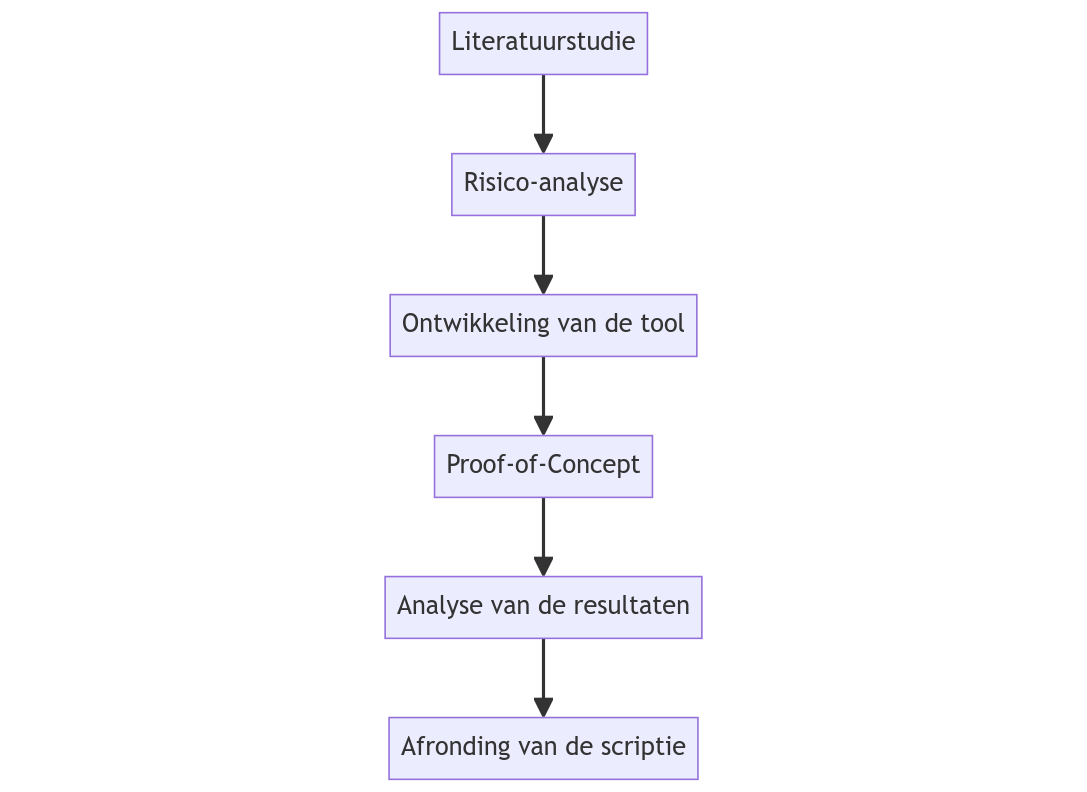
\includegraphics[width=.49\textwidth]
    {graphics/methodologie_flowchart.png}
    \caption{\label{fig:flowchart}Flowchart fasen methodologie}
\end{figure}


\subsection{Fase 1: Literatuurstudie}%
\label{sub:literatuurstudie}

De eerste fase omvat een grondige literatuurstudie die zich richt op het verzamelen van essenti\"ele configuratie en eigenschappen voor een grondige inventaris.
Daarnaast zullen ook bestaan\\de tools worden onderzocht die kunnen gebruikt worden bij het inventariseren van Linux-systemen.
Deze fase zal 2 weken in beslag nemen, en resulteert in een literatuurstudie die niet alleen de  eigenschappen van Linux-systemen identificeert die relevant zijn voor het inventaris, maar ook reeds bestaande tools die hiervoor gebruikt kunnen worden.

\subsection{Fase 2: Risico-analyse}%
\label{sub:risico_analyse}

De tweede fase richt zich op een risico-analyse, waarbij de ge\"identificeerde Linux-systeem\\eigenschappen binnen de invenaris kritisch worden ge\"evalueerd.
Via een diepgaande risico-\\analyse worden de impact van deze eigenschappen op het incidentresponseproces en hun bruikbaarheid beoordeeld.
Ook deze fase zal 2 weken in beslag nemen, en resulteert in een lijst van eigenschappen die een positieve bijdrage leveren aan het incidentresponseproces en een lijst van eigenschappen die een negatieve impact hebben.

\subsection{Fase 3: Ontwikkeling van de tool}%
\label{sub:ontwikkeling_van_de_tool}

De derde fase omvat de ontwikkeling van de tool, een Bash-script dat de eigenschappen van fase 2 gebruikt om een inventaris van het Linux-systeem op te stellen.
Het resultaat is een werkend Bash-script en zal ongeveer 3 weken in beslag nemen.

\subsection{Fase 4: Proof-of-Concept}%
\label{sub:proof_of_concept}

Na de ontwikkelingsfase volgt de Proof-of-\\Concept, waarbij een omgeving wordt opgezet met 5 Linux-servers met elk hun specifieke taak.
Deze fase zal ongeveer 1 week duren en omvat het testen van het script op de opgezette omgeving, resulterend in een inventaris van de omgeving.

\subsection{Fase 5: Analyse van de resultaten}%
\label{sub:analyse_van_de_resultaten}

Na het uitvoeren van het Proof-of-\\Concept worden de resultaten geanalyseerd.
Deze analyse vormt de basis voor de conclusie, waarbij de focus ligt op de kwaliteit en bruikbaarheid van het inventaris.
Beoordelingscriteria omvatten de volledigheid van het inventaris, de aanwezigheid van fouten en de impact op het incidentresponseproces.
Deze fase duurt 1 week.

\subsection{Fase 6: Afronding van de scriptie}%
\label{sub:afronding_van_de_scriptie}

De afsluitende fase richt zich op de voltooiing van de paper.
Ontbrekende hoofdstukken worden aangevuld, en de tekst wordt nauwkeurig nagelezen.
Het resultaat is een voltooide scriptie die voldoet aan alle vereiste normen en essenti\"ele hoofdstukken omvat.
Deze fase duurt 2 weken, maar er zal ook al aandacht aan worden besteed tijdens de voorgaande fasen.

%---------- Verwachte resultaten ----------------------------------------------
\section{Verwacht resultaat, conclusie}%
\label{sec:verwachte_resultaten}

De literatuurstudie heeft aangetoond welke systeemeigenschappen en configuratie we zouden kunnen gebruiken voor het opstellen van een inventaris.
De risico-analyse heeft kritieke eigenschappen van Linux-systemen ge\"identificeerd voor inventarisatie, waarbij een evenwicht is gezocht tussen positieve bijdragen aan het incident response proces en mogelijke negatieve effecten.

De ontwikkelde tool biedt een praktische oplossing voor het inventariseren van Linux-systemen te automatiseren.
Tijdens de Proof-of-Concept fase is aangetoond dat het script effectief is.
De inventarisatie was volledig en nauwkeurig, wat de potentie benadrukt om het incident response proces te versterken.

